\chapter{Related Work}
\section{Hashing}
\section{DMA}
These are manuals or papers that describe the DMA Engine in other works.
\subsection{Microchip PIC24F device family}
The company Microchip Inc is a provider of microcontrollers and analog semiconductors.
Among their products is the PIC24F device family \cite{microchip1}, which includes a DMA Module of its own\cite{microchip54}.
The module is located on the microcontroller data bus between the CPU and DMA-enabled peripherals, with direct access to SRAM.
The DMA controller is composed of multiple intedendent DMA channel controllers, or simply channels.
Each channel can be independently programmed to transfer data between different areas of the data RAM, move data between single or multiple addresses, use a wide range of hardware triggers to initiate transfers, and conduct programmed transactions once or many times. 
\todo{Look up the data sheet with the number of channels, if time}Numbers of channels: 
\todo{Get this confirmed!!!}The communication network in the PIC24F is the SFR-bus, which is a shared media network.
All peripherals that request data transfers are connected to this bus.
The DMA module is controlled by a number of registers.
For the module itself, there are registers for the engine control, for upper and lower address limit, and there is the data buffer.
For each channel implemented, there are registers for channel control, channel interrupt control, registers for source and destination, and there is the transaction counter. 

\subsection{Adapteva Epiphany}
The Epiphany architecture by Adapteva \todo{Compiler errors when cite name uses underscore. See note below on "epiphany"}\cite{epiphany} defines a multicore, scalable, shared-memory, parallel computing fabric.
It consists of a 2D-array of compute nodes connected by a low-latency mesh network-on-chip.
Figure \ref{fig:AdaptevaEpiphany} shows an implementation of the architecture.
As it can be seen in the figure, every node consist of a RISC CPU, local memory, a DMA Engine and a Network interface.
Every node is connected to a router.
The Epiphany architecture was designed for good performance across a broad range of applications, but excels at applications with high spatial and temporal locality of data and code.
Examples are image processing, communication, sensor signal processing, encryption and compression.
The 2D eMesh NOC that is used in this system handles traffic patterns in high-throughput real-time applications efficiently.

\todo{Hmmm.... does this sentence require that eMesh is better described? Then might as well remove}
The DMA engine is custom designed for the eMesh fabric, and operates at the same speed as the eMesh, so that  it generates a double word transaction on every clock cycle.
Every node in the Epiphany has a DMA engine each.

The main features of the DMA Engine are: \todo{Consider wether this listing REALLY is necessary} 
\begin{itemize}
    \item Two independent channels per processor node
    \item Separate specification of source/destination address configuration per descriptor and channel
    \item 2D DMA operations
    \item Flexible stride sizes
    \item DMA descriptor chaining and hardware interrupts flagging to local CPU subsystem
\end{itemize}

The DMA transfer types are: Local to external memory, vice versa, transfer to local data in slave mode, and transfer between two external sources.

DMA Descriptors are stored in local memory, and is brought into the DMA channel configuration register when register set when DMA transfer is activated.
Among the configuration are the source, destination, strides and counter.
Channel 0 has higher priority than channel 1.

\begin{figure}[h!]
    \centering
    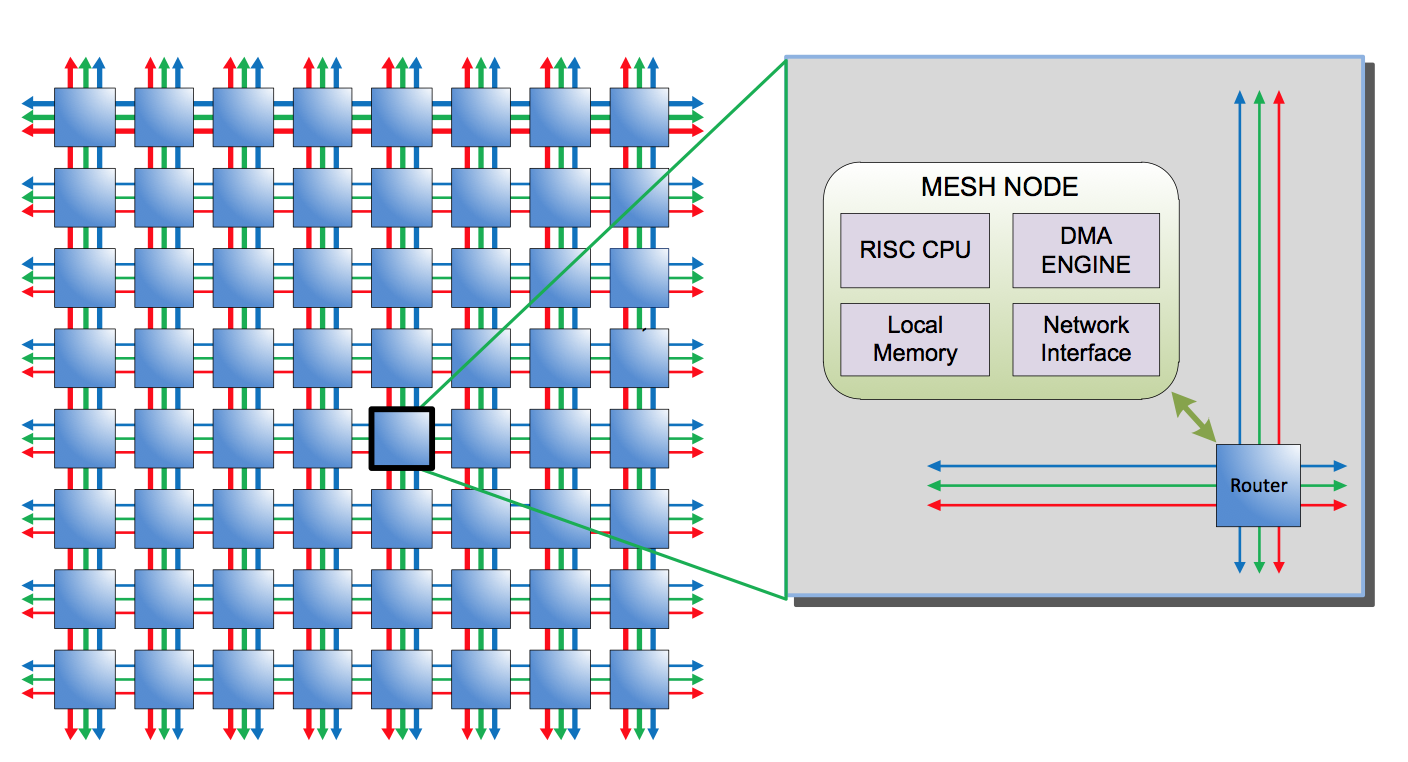
\includegraphics[width=1\textwidth]{Figures/DMA/AdaptevaEpiphany}
    \caption{An implementation of the Epiphany Architecture, as seen from \cite{epiphany}}
    \label{fig:AdaptevaEpiphany}
\end{figure}


\subsection{Cell Processor}
Kistler, Perrone and Petrini\cite{cell} takes a look at the Cell Multiprocessor, developed by IBM, Sony and Toshiba, in their paper "Cell Communication Network: Built for Speed\".
As multicores have become a major trend in computer architecture, the authors stress the need for on-chip networks that provide high performance in latency and bandwidth, if the computational power of the many anvailable processing unites are to be realized.
In this paper, the authors describes the architecture of the multiprocessor, and their experiments where they test the performance of the communication networks.
One of the main components involved in the communication is the DMA engine.

The Cell's architecture can bee seen in figure \ref{fig:CellTop}.
\begin{figure}[h!]
    \centering
    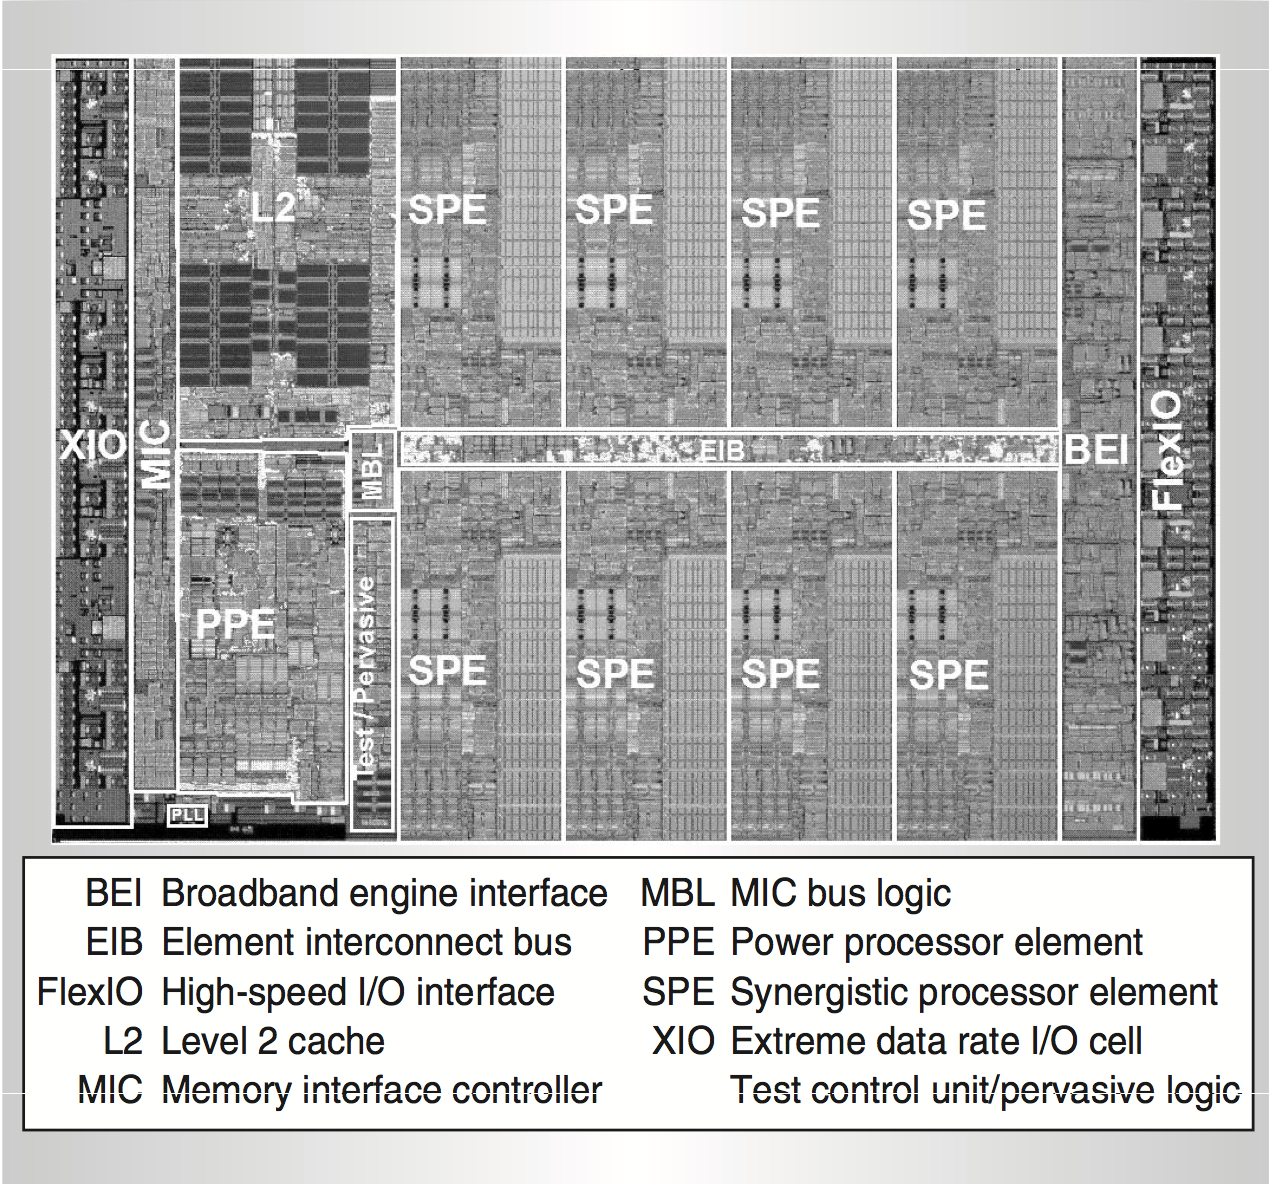
\includegraphics[width=1\textwidth]{Figures/DMA/CellTop}
    \caption{Topview of the Cell Architecture, as seen from \cite{cell}}
    \label{fig:CellTop}
\end{figure}

As can be seen in the figure, the cell consists of a Power Processor Element (PPE) and 8 specialized coprocessors called Synergetiv Processor Elements (SPE).
The PPE is the Cell's main processor.
It is a traditional 64-bit PowerPC processor core with a vector multimedia extention (VMX) unit.
It runs the operating system, and coordinates the SPEs.
Each SPE consists of a synergetic processing unit (SPU) that runs SIMD instructions, and a memory flow controller (MFC).
Each MFC consists of a DMA Controller, a memory management unit (MMU), a bus interface and an atomic unit for interfacing with other SPUs and the PPE.
The MFC connects the SPE to the element interconnect bus (EIB), which is the interconnect network that connects all the SPEs and the PPE
There are several ways of communication used for different purposes, but most of the communication between the SPU and other Cell elements is done through the DMA engine found on the MFC.

The DMA Module and the flow of a DMA transfer can be seen in figure \ref{fig:CellDMA}.
\begin{figure}[h!]
    \centering
    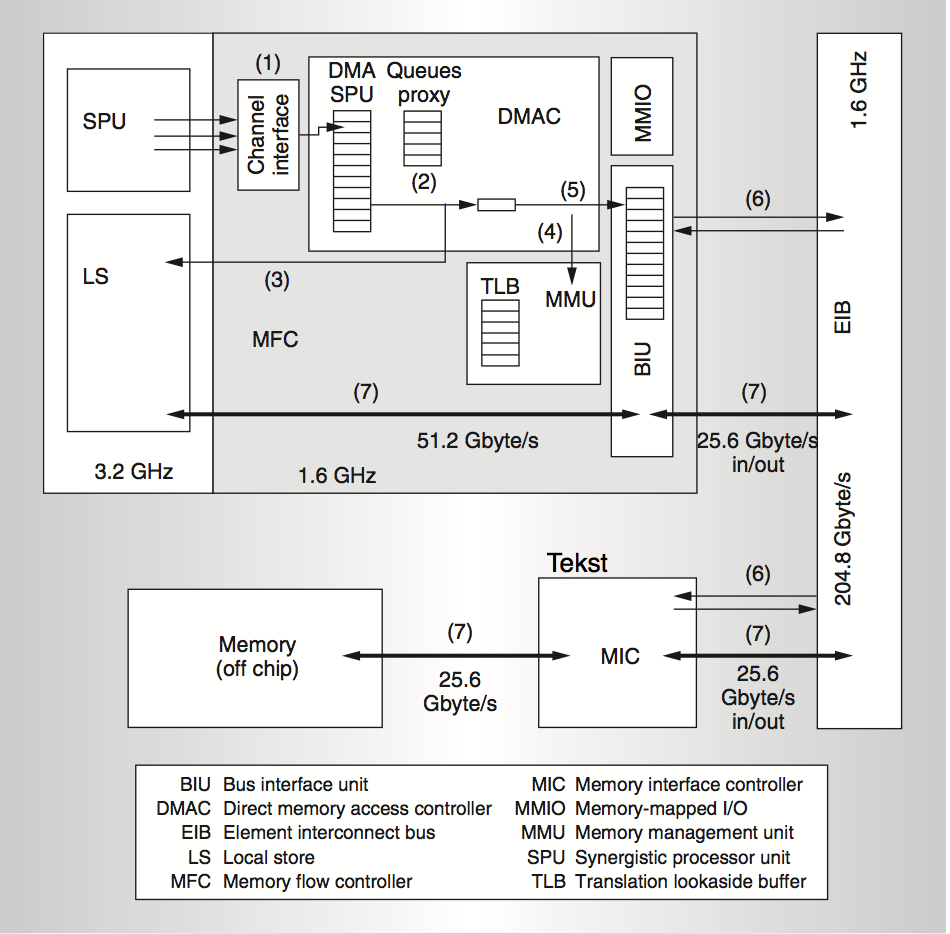
\includegraphics[width=1\textwidth]{Figures/DMA/CellDMA}
    \caption{Basic flow of a DMA transfer on the Cell, as seen from \cite{cell}}
    \label{fig:CellDMA}
\end{figure}

The commands issued for the DMA modules are gets and puts (equivalent to loads and stores).
A DMA command can also be a list command, which requests a list of multiple DMA transfer commands.
These are the steps of a DMA flow, as seen in figure \ref{fig:CellDMA}:

\begin{itemize}
    \item \textbf{1} - DMA command is placed in the MFC SPU command queue through the interface.
    \item \textbf{2} - DMAC selects a command for processing. DMA SPU queue has priority over proxy queue (commands from PPE or other devices).
    \item \textbf{3} - If DMA command is a list command that requires a list element, the DMAC must fetch the element from the local-store interface. 
    The DMA entry is updated and must be reselected.
    \item \textbf{4} - If required, due to use of virtual memory, the command is queued in the MMU, which performs the address translation (either through TLB or page table in main memory) and updates the DMA entry. 
    It must then be reselected.
    \item \textbf{5} - DMAC unrolls command.
    Unrolling means that it creates bus requests to transfer the next block of data for the command.
    Each bus request can transfer up to 128 bytes of data.
    The bus requests are queued in the to the Bus Interface Unit (BIU).
    \item \textbf{6} - The BIU selects a bus request, and issues it to the EIB, where the command is queue with others.
    If main memory is involved, the MIC must acknowledge.
    \item \textbf{7} - When the EIB has given permission, the BUI will perform the reads to local store.
    Memory from MIC is transfered by the EIB
    \item \textbf{8} - The unrolling process produces a series of bus requests for the DMA command that pipeline through the communication network.
    The DMA command remains in the SPU DMA queue until all the bus requests have been completed.
    The DMAC may still process other DMA commands.
    The SPU is notified when all bus requests are completed,, and the command is removed from the queue. 
\end{itemize}


\todo{Mention latency?}
When Kistler, Perrone and Petrini tested the performance of the communication system, they found that when using only DMA \todo{Reread and check if there were only one or more modules possible per SPE}Modules from only the highest possible bandwidth for puts and gets to local store, and puts to main memory were 22.5 GBytes/s, and gets from main memory were 15 GBytes/s, when using blocking issues.